\section{Provenance System}

In the previous section \ref{pipeline_implementation}, we described the architecture of an IoT pipeline and explained that an IoT measurement delivery pipeline consists of a set of sensors which generates measurements, which propagate along a path of several nodes. These nodes differ in several dimensions. To cope with heterogeneity of these nodes, we tried to make the architecture of the provenance system as generic as possible \ref{provenance_system}.
Provenance system consists of a daemon process and is explained below:

\begin{figure}[h]
\centering
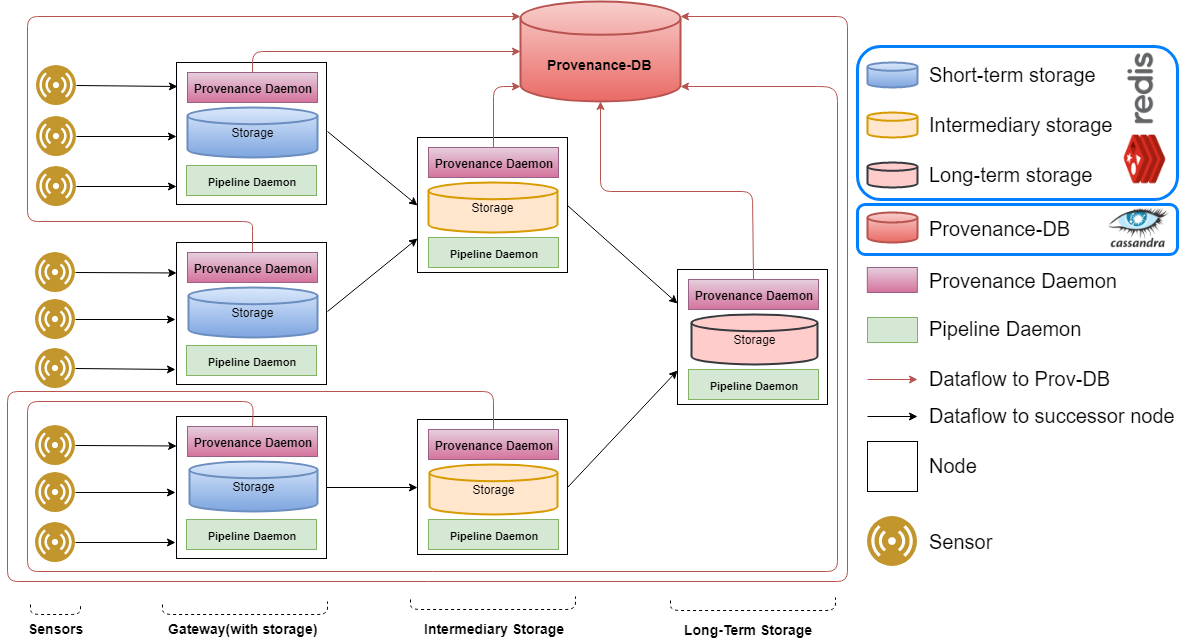
\includegraphics[width=\linewidth]{figures/provenance_system.png}\\
\caption{Provenance System}
\label{provenance_system}
\end{figure}

\subsubsection {Provenance daemon}
It runs on each node of the pipeline and as the name suggest its sole purpose is to capture provenance of the data and store it to the provenance database. Provenance daemon can be configured through the configuration file\ref{provenance_conf} and the user of the system can choose between the available metrics.
Each provenance daemon also runs a separate sub-process to capture health status of the following system components:
\begin{enumerate}
	\item Node/machine
	\item Channel - Connection between two machines.
	\item Provenance daemon
	\item Pipeline daemon
\end{enumerate}

\begin{figure}[h]
\centering
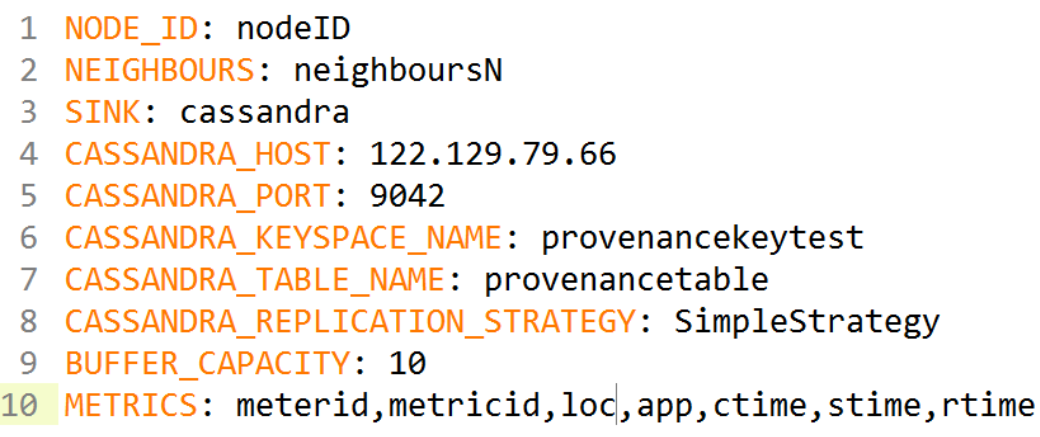
\includegraphics[width=\linewidth]{figures/conf.png}\\
\caption{Provenance System Configuration File}
\label{provenance_conf}
\end{figure}
